\subsection{Wersja 4}

\subsubsection{Opis rozwiązania}

Jest to rozszerzona wersja 3 o równoległe (na poziomie bloku) z obliczeniami pobranie kolejnych danych. Ma to spowodować złagodzenie kosztów synchronizacji -- kosztem większej ilości operacji i wymagań zasobowych.\\
Przygotowaliśmy 2 alternatywne wersje wyprzedzającego pobrania:

\begin{enumerate}[(a)]

\item Pobranie do rejestru

W tej wersji dane potrzebne w następnej iteracji pobierane są do rejestru.

\lstinputlisting[caption=Mnożenie macierzy kwadratowych na GPU -- wersja 4 z pobraniem do rejestru.]{./code/matrix_multiplication_4a.cpp}

\item Pobranie do pamięci współdzielonej

W tej wersji dane potrzebne w następnej iteracji pobierane są do pamięci współdzielonej -- ilość wykorzystanej pamięci współdzielonej przez blok wzrasta dwukrotnie.

\lstinputlisting[caption=Mnożenie macierzy kwadratowych na GPU -- wersja 4 z pobraniem do pamięci współdzielonej.]{./code/matrix_multiplication_4b.cpp}

\end{enumerate}

\subsubsection{Teoretyczna zajętość SM}

\begin{enumerate}[(a)]

\begin{minipage}[c]{\textwidth}

\item Pobranie do rejestru

\begin{center}
\begin{table}[H]
\centering
\resizebox{\textwidth}{!}{%
\begin{tabularx}{1.1\textwidth}{|c|c|>{\centering}X|>{\centering}X|c|}
\hline
\multicolumn{2}{|c|}{\multirow{2}{*}{Kryterium}} & \multicolumn{2}{c|}{Teoretyczna wartość} & \multirow{2}{*}{Limit GPU} \\ \cline{3-4}
\multicolumn{2}{|c|}{} & 8x8 & 16x16 & \\ \hline
\multirow{4}{*}{Zajętość SM} & Aktywne bloki & 8 & 4 & 8 \\ \cline{2-5}
& Aktywne warpy & 16 & 32 & 32 \\ \cline{2-5}
& Aktywne wątki & 512 & 1024 & 1024 \\ \cline{2-5}
& Zajętość & 50\% & 100\% & 100\% \\ \hline
\multirow{3}{*}{Warpy} & Wątki/Blok & 64 & 256 & 512 \\ \cline{2-5}
& Warpy/Blok & 2 & 8 & 16 \\ \cline{2-5}
& Limit bloków & 16 & \textcolor{red}{\textbf{4}} & 8 \\ \hline
\multirow{3}{*}{Rejestry} & Rejestry/Wątek & 13 & 13 & 128 \\ \cline{2-5}
& Rejestry/Blok & 1024 & 3584 & 16384 \\ \cline{2-5}
& Limit bloków & 16 & \textcolor{red}{\textbf{4}} & 8 \\ \hline
Pamięć & Pamięć współdzielona/Blok & 556 & 2092 & 16384 \\ \cline{2-5}
współdzielona & Limit bloków & 16 & 6 & 8 \\ \hline
\end{tabularx}
}
\caption{Teoretyczna zajętość SM -- wersja 4. z pobraniem do rejestru.}
\end{table}
\end{center}

Podobnie jak dla poprzednich wersji, dla bloku 8x8 limitem okazuje się być maksymalna ilość warpów na SM, stąd zajętość $ 16 / 32 = 50\% $. \\
Dla macierzy 16x16 limitem są warpy i rejestry. Przypada odpowiednio $ 8 $ warpów na blok, co daje limit $ 4 $ aktywnych bloków. $ 3584 $ rejestrów na blok również daje limit $ 4 $ aktywnych bloków. Zajętość dla bloku 16x16 wynosi $ 100\% $. \\

\end{minipage}

\begin{minipage}[c]{\textwidth}

\item Pobranie do pamięci współdzielonej

\begin{center}
\begin{table}[H]
\centering
\resizebox{\textwidth}{!}{%
\begin{tabularx}{1.1\textwidth}{|c|c|>{\centering}X|>{\centering}X|c|}
\hline
\multicolumn{2}{|c|}{\multirow{2}{*}{Kryterium}} & \multicolumn{2}{c|}{Teoretyczna wartość} & \multirow{2}{*}{Limit GPU} \\ \cline{3-4}
\multicolumn{2}{|c|}{} & 8x8 & 16x16 & \\ \hline
\multirow{4}{*}{Zajętość SM} & Aktywne bloki & 8 & 3 & 8 \\ \cline{2-5}
& Aktywne warpy & 16 & 24 & 32 \\ \cline{2-5}
& Aktywne wątki & 512 & 768 & 1024 \\ \cline{2-5}
& Zajętość & 50\% & 75\% & 100\% \\ \hline
\multirow{3}{*}{Warpy} & Wątki/Blok & 64 & 256 & 512 \\ \cline{2-5}
& Warpy/Blok & 2 & 8 & 16 \\ \cline{2-5}
& Limit bloków & 16 & 4 & 8 \\ \hline
\multirow{3}{*}{Rejestry} & Rejestry/Wątek & 14 & 14 & 128 \\ \cline{2-5}
& Rejestry/Blok & 1024 & 3584 & 16384 \\ \cline{2-5}
& Limit bloków & 16 & 4 & 8 \\ \hline
Pamięć & Pamięć współdzielona/Blok & 1068 & 4140 & 16384 \\ \cline{2-5}
współdzielona & Limit bloków & 16 & \textcolor{red}{\textbf{3}} & 8 \\ \hline
\end{tabularx}
}
\caption{Teoretyczna zajętość SM -- wersja 4. z pobraniem do pamięci współdzielonej.}
\end{table}
\end{center}

Również w tym przypadku dla bloku 8x8 limitem okazuje się być maksymalna ilość warpów na SM, stąd zajętość $ 16 / 32 = 50\% $. \\
Dla macierzy 16x16 limitem jest pamięć współdzielona. $4140$ bajtów na blok daje limit $3$ aktywnych bloków. W porównaniu z poprzednimi wersjami zajętość SM dla bloku 16x16 spada i wynosi $ 75\% $. \\

\end{minipage}

\end{enumerate}

\subsubsection{Wyniki pomiarów}

\paragraph{Czas trwania obliczeń}

\begin{minipage}[c]{\textwidth}

\begin{enumerate}[(a)]

\item Pobranie do rejestru

\begin{figure}[H]

  \begin{minipage}[c]{0.46\textwidth}
  \centering
  \resizebox{\textwidth}{!}{%
  \begin{tabular}{|c|c|c|}
  \hline
  \multirow{2}{*}{Rozmiar macierzy} & \multicolumn{2}{c|}{Rozmiar bloku} \\ \cline{2-3}
  & 8x8 & 16x16 \\ \hline
  128x128 & 0.145 & 0.091 \\ \hline
  256x256 & 0.940 & 0.525 \\ \hline
  384x384 & 3.062 & 1.632 \\ \hline
  512x512 & 7.093 & 3.809 \\ \hline
  640x640 & 13.950 & 7.356 \\ \hline
  \end{tabular}
  \captionlistentry[table]{Czas obliczeń [ms] -- wersja 4. z pobraniem do rejestru.}
  }

  \end{minipage}
  \qquad
  \begin{minipage}[c]{0.46\textwidth}
  \centering

  \resizebox{\textwidth}{!}{%
    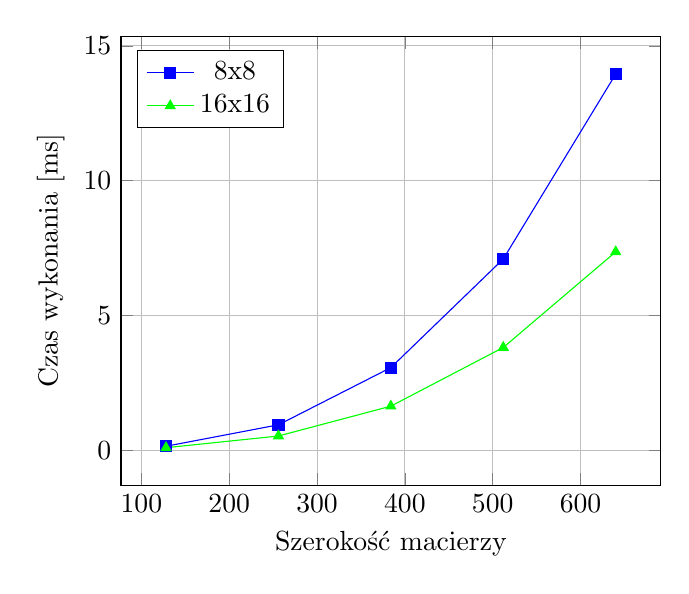
\begin{tikzpicture}
      \begin{axis}[
        xlabel=Szerokość macierzy,
        ylabel={Czas wykonania [ms]},
        legend pos=north west,
        grid=both
      ]

      \addplot[color=blue,mark=square*] coordinates {%
        (128, 0.145)
        (256, 0.940)
        (384, 3.062)
        (512, 7.093)
        (640, 13.950)
      };
      \addlegendentry{8x8}

      \addplot[color=green,mark=triangle*] coordinates {%
        (128, 0.091)
        (256, 0.525)
        (384, 1.632)
        (512, 3.809)
        (640, 7.356)
      };
      \addlegendentry{16x16}

      \end{axis}%
    \end{tikzpicture}%
  }

  \end{minipage}

  \captionsetup{labelformat=andtable}
  \caption{Zależność pomiędzy czasem obliczeń a rozmiarem macierzy -- wersja 4. z pobraniem do rejestru.}
\end{figure}

\item Pobranie do pamięci współdzielonej

\begin{figure}[H]

  \begin{minipage}[c]{0.46\textwidth}
  \centering
  \resizebox{\textwidth}{!}{%
  \begin{tabular}{|c|c|c|}
  \hline
  \multirow{2}{*}{Rozmiar macierzy} & \multicolumn{2}{c|}{Rozmiar bloku} \\ \cline{2-3}
  & 8x8 & 16x16 \\ \hline
  128x128 & 0.156 & 0.093 \\ \hline
  256x256 & 1.069 & 0.610 \\ \hline
  384x384 & 3.461 & 1.956 \\ \hline
  512x512 & 8.023 & 4.430 \\ \hline
  640x640 & 15.838 & 8.606 \\ \hline
  \end{tabular}
  \captionlistentry[table]{Czas obliczeń [ms] -- wersja 4. z pobraniem do pamięci współdzielonej.}
  }

  \end{minipage}
  \qquad
  \begin{minipage}[c]{0.46\textwidth}
  \centering

  \resizebox{\textwidth}{!}{%
    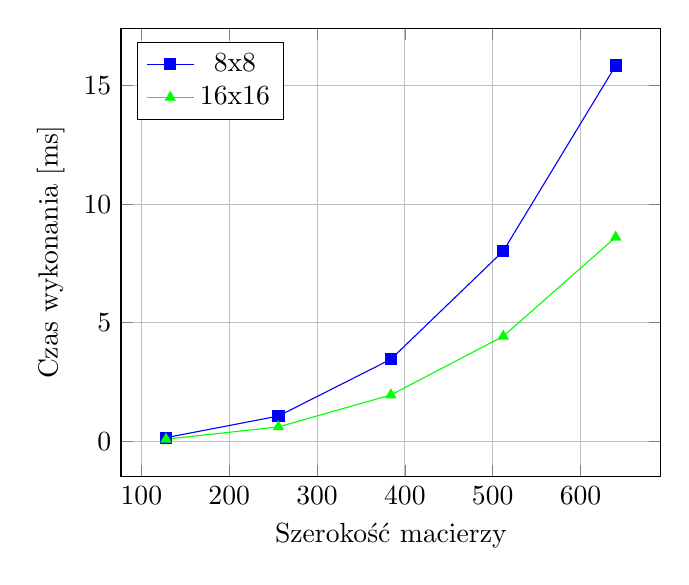
\begin{tikzpicture}
      \begin{axis}[
        xlabel=Szerokość macierzy,
        ylabel={Czas wykonania [ms]},
        legend pos=north west,
        grid=both
      ]

      \addplot[color=blue,mark=square*] coordinates {%
        (128, 0.156)
        (256, 1.069)
        (384, 3.461)
        (512, 8.023)
        (640, 15.838)
      };
      \addlegendentry{8x8}

      \addplot[color=green,mark=triangle*] coordinates {%
        (128, 0.093)
        (256, 0.610)
        (384, 1.956)
        (512, 4.430)
        (640, 8.606)
      };
      \addlegendentry{16x16}

      \end{axis}%
    \end{tikzpicture}%
  }
  
  \end{minipage}

  \captionsetup{labelformat=andtable}
  \caption{Zależność pomiędzy czasem obliczeń a rozmiarem macierzy -- wersja 4. z pobraniem do pamięci współdzielonej.}

\end{figure}

\end{enumerate}

\end{minipage}

\begin{minipage}[c]{\textwidth}

\paragraph{Ilość operacji zmiennoprzecinkowych na sekundę}

\begin{enumerate}[(a)]

\item Pobranie do rejestru

\begin{figure}[H]

  \begin{minipage}[c]{0.46\textwidth}
  \centering
  \resizebox{\textwidth}{!}{%
  \begin{tabular}{|c|c|c|}
  \hline
  \multirow{2}{*}{Rozmiar macierzy} & \multicolumn{2}{c|}{Rozmiar bloku} \\ \cline{2-3}
  & 8x8 & 16x16 \\ \hline
  128x128 & 28.953 & 45.894 \\ \hline
  256x256 & 35.697 & 63.856 \\ \hline
  384x384 & 36.987 & 69.405 \\ \hline
  512x512 & 37.844 & 70.472 \\ \hline
  640x640 & 37.583 & 71.269 \\ \hline
  \end{tabular}
  \captionlistentry[table]{Ilość operacji zmiennoprzecinkowych na sekundę (GFLOPS) -- wersja 4. z pobraniem do rejestru.}
  }

  \end{minipage}
  \qquad
  \begin{minipage}[c]{0.46\textwidth}
  \centering

  \resizebox{\textwidth}{!}{%
    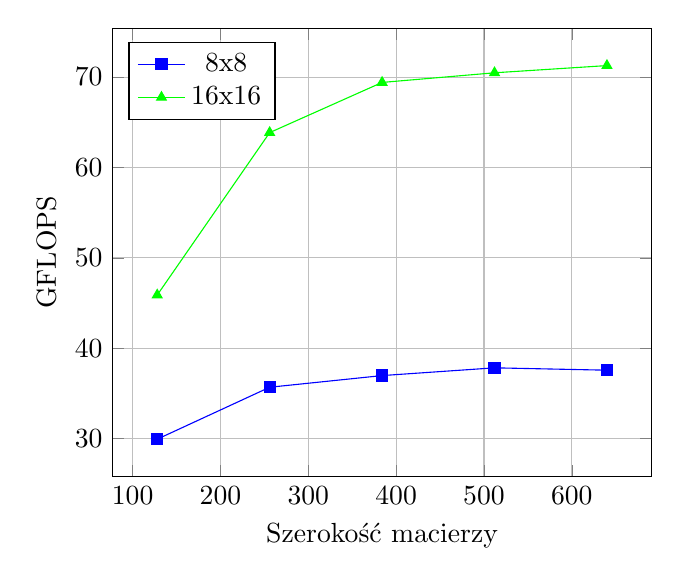
\begin{tikzpicture}
      \begin{axis}[
        xlabel=Szerokość macierzy,
        ylabel={GFLOPS},
        legend pos=north west,
        grid=both
      ]

      \addplot[color=blue,mark=square*] coordinates {%
        (128, 29.953)
        (256, 35.697)
        (384, 36.987)
        (512, 37.844)
        (640, 37.583)
      };
      \addlegendentry{8x8}

      \addplot[color=green,mark=triangle*] coordinates {%
        (128, 45.894)
        (256, 63.856)
        (384, 69.405)
        (512, 70.472)
        (640, 71.269)
      };
      \addlegendentry{16x16}

      \end{axis}%
    \end{tikzpicture}%
  }

  \end{minipage}

  \captionsetup{labelformat=andtable}
  \caption{Zależność pomiędzy ilością operacji zmiennoprzecinkowych na sekundę a rozmiarem macierzy -- wersja 4. z pobraniem do rejestru.}

\end{figure}

\item Pobranie do pamięci współdzielonej

\begin{figure}[H]

  \begin{minipage}[c]{0.46\textwidth}
  \centering
  \resizebox{\textwidth}{!}{%
  \begin{tabular}{|c|c|c|}
  \hline
  \multirow{2}{*}{Rozmiar macierzy} & \multicolumn{2}{c|}{Rozmiar bloku} \\ \cline{2-3}
  & 8x8 & 16x16 \\ \hline
  128x128 & 26.892 & 45.291 \\ \hline
  256x256 & 31.394 & 55.012 \\ \hline
  384x384 & 32.723 & 57.902 \\ \hline
  512x512 & 33.458 & 60.593 \\ \hline
  640x640 & 33.103 & 60.919 \\ \hline
  \end{tabular}
  \captionlistentry[table]{Ilość operacji zmiennoprzecinkowych na sekundę (GFLOPS) -- wersja 4. z pobraniem do pamięci współdzielonej.}
  }

  \end{minipage}
  \qquad
  \begin{minipage}[c]{0.46\textwidth}
  \centering

  \resizebox{\textwidth}{!}{%
    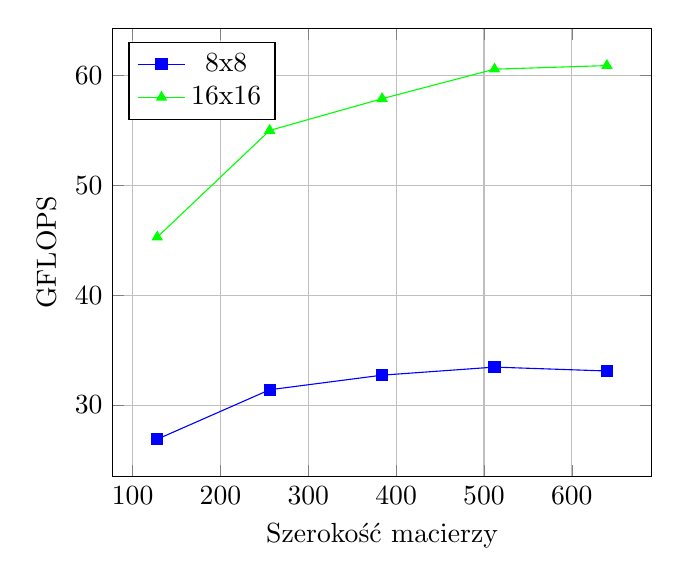
\begin{tikzpicture}
      \begin{axis}[
        xlabel=Szerokość macierzy,
        ylabel={GFLOPS},
        legend pos=north west,
        grid=both
      ]

      \addplot[color=blue,mark=square*] coordinates {%
        (128, 26.892)
        (256, 31.394)
        (384, 32.723)
        (512, 33.458)
        (640, 33.103)
      };
      \addlegendentry{8x8}

      \addplot[color=green,mark=triangle*] coordinates {%
        (128, 45.291)
        (256, 55.012)
        (384, 57.902)
        (512, 60.593)
        (640, 60.919)
      };
      \addlegendentry{16x16}

      \end{axis}%
    \end{tikzpicture}%
  }
  
  \end{minipage}

  \captionsetup{labelformat=andtable}
  \caption{Zależność pomiędzy ilością operacji zmiennoprzecinkowych na sekundę a rozmiarem macierzy -- wersja 5. z pobraniem do pamięci współdzielonej.}

\end{figure}

\end{enumerate}

\end{minipage}

\paragraph{Ilość instrukcji na sekundę}

\begin{minipage}[c]{\textwidth}

\begin{enumerate}[(a)]

\item Pobranie do rejestru

\begin{figure}[H]

  \begin{minipage}[c]{0.46\textwidth}
  \centering
  \resizebox{\textwidth}{!}{%
  \begin{tabular}{|c|c|c|c|}
  \hline
  \multirow{2}{*}{Rozmiar macierzy} & \multicolumn{2}{c|}{Rozmiar bloku} \\ \cline{2-3}
  & 8x8 & 16x16 \\ \hline
  128x128 & 0.1448 & 0.1639 \\ \hline
  256x256 & 0.1787 & 0.2665 \\ \hline
  384x384 & 0.1821 & 0.3020 \\ \hline
  512x512 & 0.1848 & 0.2983 \\ \hline
  640x640 & 0.1815 & 0.3013 \\ \hline
  \end{tabular}
  \captionlistentry[table]{Ilość instrukcji wykonana na sekundę (GIPS) -- wersja 4. z pobraniem do rejestru.}
  }

  \end{minipage}
  \qquad
  \begin{minipage}[c]{0.46\textwidth}
  \centering

  \resizebox{\textwidth}{!}{%
    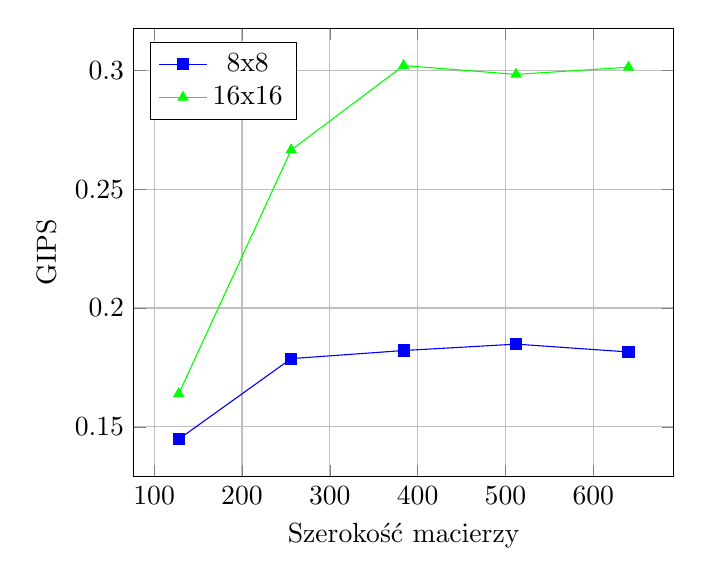
\begin{tikzpicture}
      \begin{axis}[
        xlabel=Szerokość macierzy,ylabel={GIPS},legend pos= north west,grid=both]

      \addplot[color=blue,mark=square*] coordinates {%
        (128, 0.1448)
        (256, 0.1787)
        (384, 0.1821)
        (512, 0.1848)
        (640, 0.1815)
      };
      \addlegendentry{8x8}

      \addplot[color=green,mark=triangle*] coordinates {%
        (128, 0.1639)
        (256, 0.2665)
        (384, 0.3020)
        (512, 0.2983)
        (640, 0.3013)
      };
      \addlegendentry{16x16}

      \end{axis}%
    \end{tikzpicture}%
  }
  \end{minipage}
  \captionsetup{labelformat=andtable}
  \caption{Zależność pomiędzy ilością instrukcji wykonanych na sekundę a rozmiarem macierzy -- wersja 4. z pobraniem do rejestru.}

\end{figure}

\item Pobranie do pamięci współdzielonej

\begin{figure}[H]

  \begin{minipage}[c]{0.46\textwidth}
  \centering
  \resizebox{\textwidth}{!}{%
  \begin{tabular}{|c|c|c|c|}
  \hline
  \multirow{2}{*}{Rozmiar macierzy} & \multicolumn{2}{c|}{Rozmiar bloku} \\ \cline{2-3}
  & 8x8 & 16x16 \\ \hline
  128x128 & 0.1918 & 0.2248 \\ \hline
  256x256 & 0.1904 & 0.2944 \\ \hline
  384x384 & 0.1934 & 0.2812 \\ \hline
  512x512 & 0.1958 & 0.2932 \\ \hline
  640x640 & 0.1927 & 0.2920 \\ \hline
  \end{tabular}
  \captionlistentry[table]{Ilość instrukcji wykonana na sekundę (GIPS) -- wersja 4. z pobraniem do pamięci współdzielonej.}
  }

  \end{minipage}
  \qquad
  \begin{minipage}[c]{0.46\textwidth}
  \centering

  \resizebox{\textwidth}{!}{%
    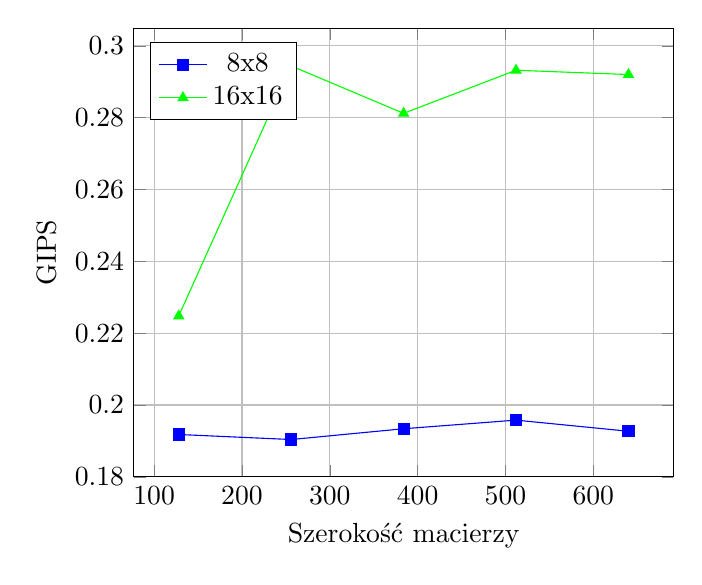
\begin{tikzpicture}
      \begin{axis}[
        xlabel=Szerokość macierzy,
        ylabel={GIPS},
        legend pos=north west,
        grid=both
      ]

      \addplot[color=blue,mark=square*] coordinates {%
        (128, 0.1918)
        (256, 0.1904)
        (384, 0.1934)
        (512, 0.1958)
        (640, 0.1927)
      };
      \addlegendentry{8x8}

      \addplot[color=green,mark=triangle*] coordinates {%
        (128, 0.2248)
        (256, 0.2944)
        (384, 0.2812)
        (512, 0.2932)
        (640, 0.2920)
      };
      \addlegendentry{16x16}

      \end{axis}%
    \end{tikzpicture}%
  }
  
  \end{minipage}

  \captionsetup{labelformat=andtable}
  \caption{Zależność pomiędzy ilością instrukcji wykonanych na sekundę a rozmiarem macierzy -- wersja 4. z pobraniem do pamięci współdzielonej.}
\end{figure}

\end{enumerate}

\end{minipage}

\paragraph{CGMA}

\begin{minipage}[c]{\textwidth}

\begin{enumerate}[(a)]

\item Pobranie do rejestru

\begin{figure}[H]

  \begin{minipage}[c]{0.46\textwidth}
  \centering
  \resizebox{\textwidth}{!}{%
  \begin{tabular}{|c|c|c|c|}
  \hline
  \multirow{2}{*}{Rozmiar macierzy} & \multicolumn{2}{c|}{Rozmiar bloku} \\ \cline{2-3}
  & 8x8 & 16x16 \\ \hline
  128x128 & 120.471 & 485.452 \\ \hline
  256x256 & 124.121 & 489.531 \\ \hline
  384x384 & 125.388 & 491.520 \\ \hline
  512x512 & 125.908 & 498.432 \\ \hline
  640x640 & 126.499 & 500.764 \\ \hline
  \end{tabular}
  \captionlistentry[table]{Stosunek ilości operacji zmiennoprzecinkowych do ilości operacji odczytu/zapisu z pamięci globalnej -- wersja 4. z pobraniem do rejestru.}
  }

  \end{minipage}
  \qquad
  \begin{minipage}[c]{0.46\textwidth}
  \centering

  \resizebox{\textwidth}{!}{%
    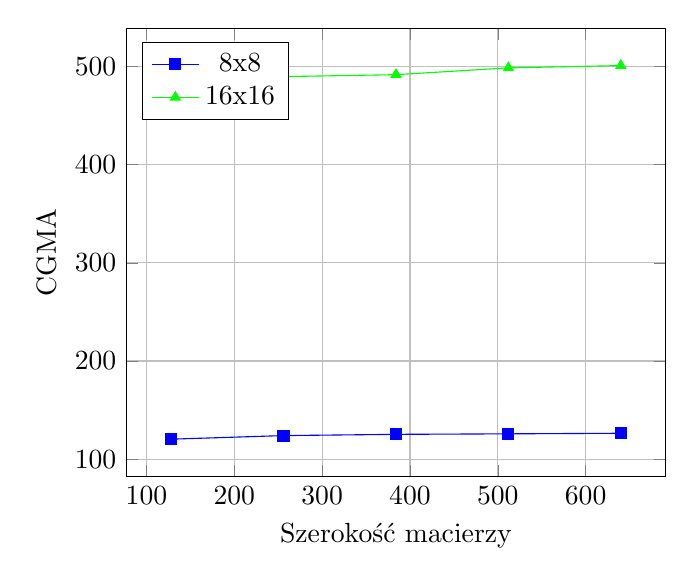
\begin{tikzpicture}
      \begin{axis}[
        xlabel=Szerokość macierzy,ylabel={CGMA},legend pos= north west,grid=both]

      \addplot[color=blue,mark=square*] coordinates {%
        (128, 120.471)
        (256, 124.121)
        (384, 125.388)
        (512, 125.908)
        (640, 126.499)
      };
      \addlegendentry{8x8}

      \addplot[color=green,mark=triangle*] coordinates {%
        (128, 485.452)
        (256, 489.531)
        (384, 491.520)
        (512, 498.432)
        (640, 500.764)
      };
      \addlegendentry{16x16}

      \end{axis}%
    \end{tikzpicture}%
  }
  \end{minipage}
  \captionsetup{labelformat=andtable}
  \caption{Zależność CGMA od rozmiaru macierzy -- wersja 4. z pobraniem do rejestru}

\end{figure}

\item Pobranie do pamięci współdzielonej

\begin{figure}[H]

  \begin{minipage}[c]{0.46\textwidth}
  \centering
  \resizebox{\textwidth}{!}{%
  \begin{tabular}{|c|c|c|c|}
  \hline
  \multirow{2}{*}{Rozmiar macierzy} & \multicolumn{2}{c|}{Rozmiar bloku} \\ \cline{2-3}
  & 8x8 & 16x16 \\ \hline
  128x128 & 115.076 & 520.127 \\ \hline
  256x256 & 124.608 & 481.882 \\ \hline
  384x384 & 125.388 & 494.957 \\ \hline
  512x512 & 126.031 & 496.485 \\ \hline
  640x640 & 126.657 & 498.267 \\ \hline
  \end{tabular}
  \captionlistentry[table]{Stosunek ilości operacji zmiennoprzecinkowych do ilości operacji odczytu/zapisu z pamięci globalnej -- wersja 4. z pobraniem do rejestru.}
  }

  \end{minipage}
  \qquad
  \begin{minipage}[c]{0.46\textwidth}
  \centering

  \resizebox{\textwidth}{!}{%
    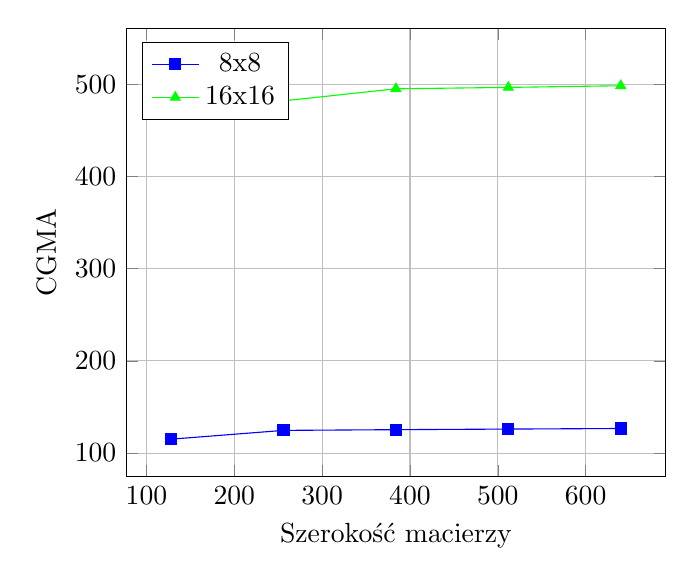
\begin{tikzpicture}
      \begin{axis}[
        xlabel=Szerokość macierzy,
        ylabel={CGMA},
        legend pos=north west,
        grid=both
      ]

      \addplot[color=blue,mark=square*] coordinates {%
        (128, 115.076)
        (256, 124.608)
        (384, 125.388)
        (512, 126.031)
        (640, 126.657)
      };
      \addlegendentry{8x8}

      \addplot[color=green,mark=triangle*] coordinates {%
        (128, 520.127)
        (256, 481.882)
        (384, 494.957)
        (512, 496.485)
        (640, 498.267)
      };
      \addlegendentry{16x16}

      \end{axis}%
    \end{tikzpicture}%
  }
  
  \end{minipage}

  \captionsetup{labelformat=andtable}
  \caption{Zależność CGMA od rozmiaru macierzy -- wersja 4. z pobraniem do pamięci współdzielonej.}
\end{figure}

\end{enumerate}

\end{minipage}

